%
% analyse.tex
%
% (c) 2020 Prof Dr Andreas Müller, Hochschule Rapperswil
%
\begin{frame}
\frametitle{Konvergenz/Divergenz}
\begin{center}
\begin{columns}[t]
\begin{column}{0.48\hsize}
\only<1-2>{
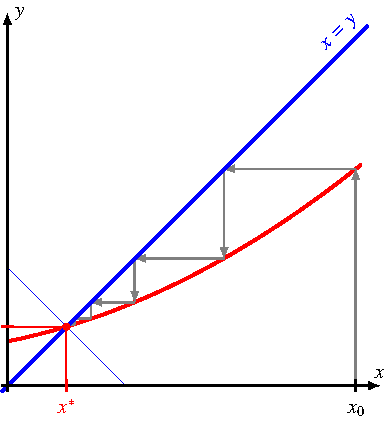
\includegraphics[width=\hsize]{../../buch/chapters/10-arithmetik/figures/normal.pdf}}
\only<3-4>{
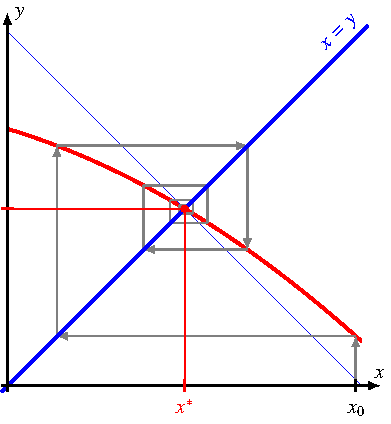
\includegraphics[width=\hsize]{../../buch/chapters/10-arithmetik/figures/negativ.pdf}}
\only<5>{
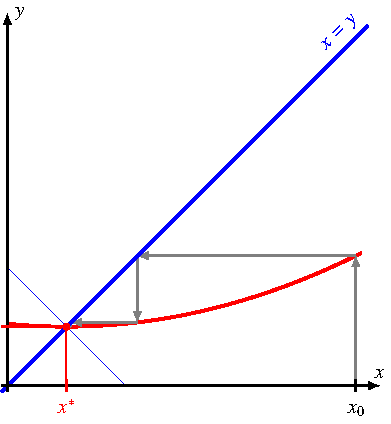
\includegraphics[width=\hsize]{../../buch/chapters/10-arithmetik/figures/quadratisch.pdf}}
\only<6-7>{
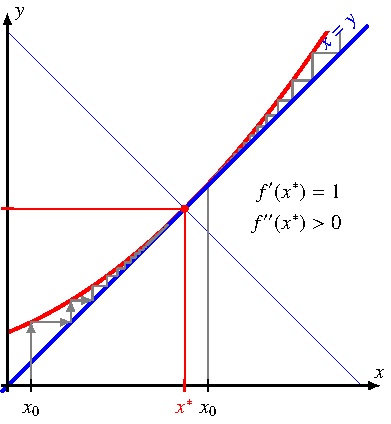
\includegraphics[width=\hsize]{../../buch/chapters/10-arithmetik/figures/m1qp.pdf}}
\only<8-9>{
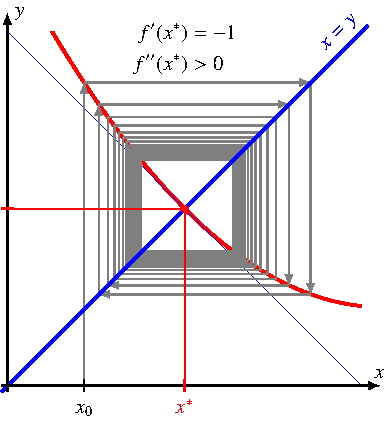
\includegraphics[width=\hsize]{../../buch/chapters/10-arithmetik/figures/mnqp.pdf}}
\only<10-11>{
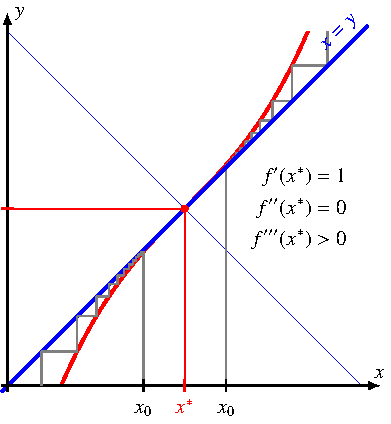
\includegraphics[width=\hsize]{../../buch/chapters/10-arithmetik/figures/m1kp.pdf}}
\only<12-13>{
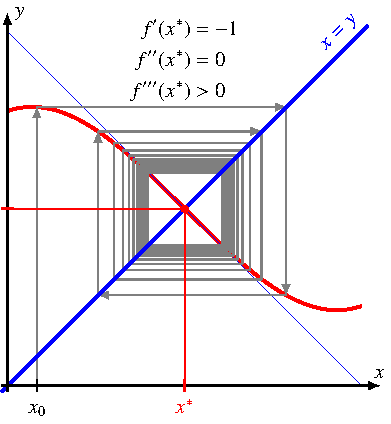
\includegraphics[width=\hsize]{../../buch/chapters/10-arithmetik/figures/mnkp.pdf}}
\end{column}
\begin{column}{0.48\hsize}
\only<2-3>{
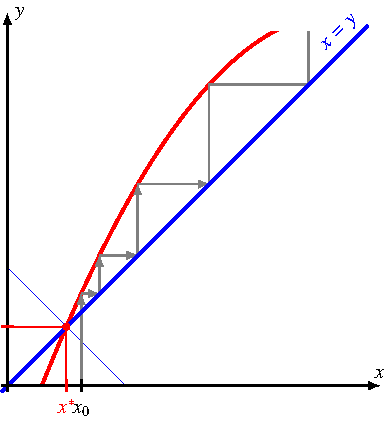
\includegraphics[width=\hsize]{../../buch/chapters/10-arithmetik/figures/divergent.pdf}}
\only<4>{
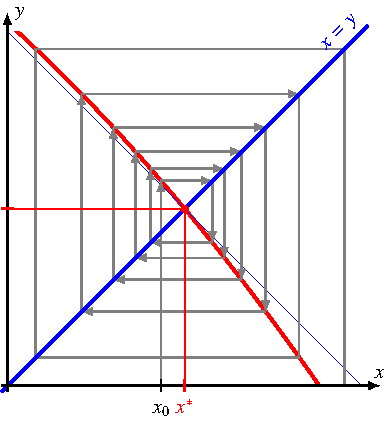
\includegraphics[width=\hsize]{../../buch/chapters/10-arithmetik/figures/negdiv.pdf}}
\only<7>{
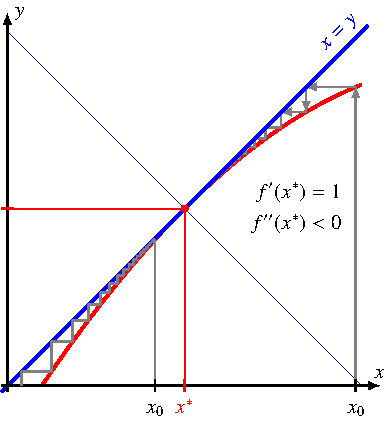
\includegraphics[width=\hsize]{../../buch/chapters/10-arithmetik/figures/m1qn.pdf}}
\only<9>{
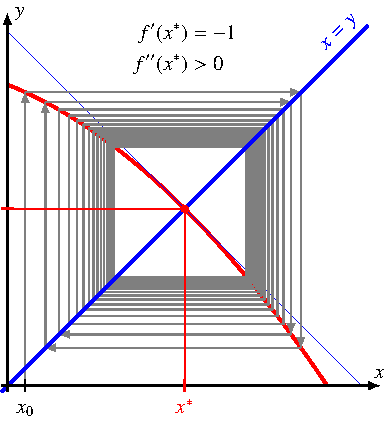
\includegraphics[width=\hsize]{../../buch/chapters/10-arithmetik/figures/mnqn.pdf}}
\only<11>{
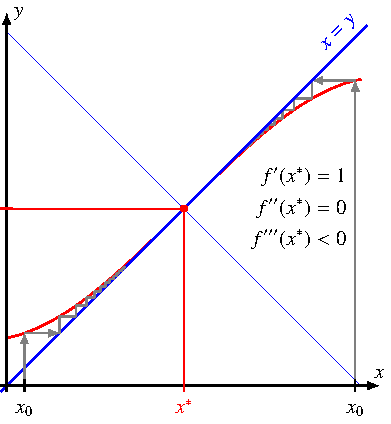
\includegraphics[width=\hsize]{../../buch/chapters/10-arithmetik/figures/m1kn.pdf}}
\only<13>{
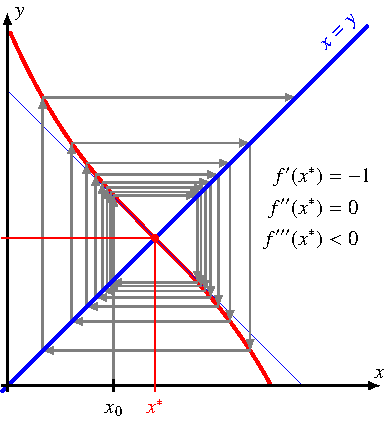
\includegraphics[width=\hsize]{../../buch/chapters/10-arithmetik/figures/mnkn.pdf}}
\end{column}
\end{columns}
\end{center}
\end{frame}
